\documentclass[pdf, hyperref={unicode}, aspectratio=169]{beamer}

\usepackage{diploma-slides-latex-template/styles}
\setbeamertemplate{navigation symbols}{}

\usepackage{nicematrix}
\usepackage{tikz}
\usetikzlibrary{arrows, positioning}

% \usepackage{grfext}

% \AtBeginDocument{%
%   \PrependGraphicsExtensions*{
%     .png,.PNG,
%     .pdf,.PDF
%   }%
% }

\title{Разреженная идентификация нелинейных динамических систем}

\subtitle{Выпускная квалификационная работа бакалавра}

\pdfstringdefDisableCommands{
  \def\\{}
  \def\,{}
  \def\textbf#1{<#1>}
}

\author[Бирюков Виктор Владимирович]
{
  \textbf{Студент группы М8О-407Б-19:} Бирюков Виктор Владимирович\\
  \ \textbf{Научный руководитель:} д.ф.-м.н., проф., проф. каф. 806 Д.\,Л.\,Ревизников
}

\institute[Московский авиационный институт]
{
  Московский авиационный институт (национальный исследовательский университет)\\
  Институт № 8 «Компьютерные науки и прикладная математика»\\
  Кафедра № 806 «Вычислительная математика и программирование» 
}

\date{Москва --- \the\year}

\logo{
\includegraphics[height=1cm]{img/mai}}

\begin{document}

\frame{\titlepage}

\begin{frame}
\frametitle{Актуальность темы}

\begin{itemize}
  \item Динамические системы описывают большое количество различных процессов.
  \item Задача извлечения закономерностей из большого объема шумных данных может превышать возможности человека.
  \item Знание динамической системы, лежащей за данными, позволит использовать соответствующий математический аппарат как часть анализа данных.
\end{itemize}
\end{frame}


\begin{frame}
\frametitle{Цель и задача работы}

\textbf{Цель} --- идентификация систем обыкновенных дифференциальных уравнений первого порядка на основе потенциально шумных данных.

\textbf{Задачи:}
\begin{itemize}
  \item Реализация алгоритма идентификации.
  \item Выбор и реализация алгоритмов разреженной регрессии.
  \item Выбор и реализация алгоритмов дифференцирования шумных данных.
  \item Сравнение различных методов дифференцирования и регрессии.
  \item Тестирование алгоритма идентификации на известных системах ОДУ.
\end{itemize}
\end{frame}


\begin{frame}
\frametitle{Постановка задачи}

\textbf{Дано:}
\begin{itemize}
  \item Входные данные представляют из себя массив значений некоторых величин
  \item Данные могут содержать некоторую шумовую компоненту
  \item Предполагается, что замеры величин производились через равные промежутки времени
\end{itemize}

\textbf{Необходимо} разработать алгоритм, при помощи которого можно получить динамическую систему (систему ОДУ), которая описывает эволюцию заданных величин.
\end{frame}


\begin{frame}
\frametitle{Алгоритм решения задачи}

\small
\vspace{-\abovedisplayskip}
\begin{equation*}
  \begin{gathered}
  \begin{bNiceMatrix}[first-row]
  x & y & z \\
  x_1 & y_1 & z_1 \\
  x_2 & y_2 & z_2 \\
  \vdots & \vdots & \vdots \\
  x_n & y_n & z_n
  \end{bNiceMatrix}\\
  X
  \end{gathered}
  \qquad
  \begin{gathered}
  \begin{bNiceMatrix}[first-row]
  \dot{x} & \dot{y} & \dot{z} \\
  \dot{x_1} & \dot{y_1} & \dot{z_1} \\
  \dot{x_2} & \dot{y_2} & \dot{z_2} \\
  \vdots & \vdots & \vdots \\
  \dot{x_n} & \dot{y_n} & \dot{z_n}
  \end{bNiceMatrix}\\
  \dot{X}
  \end{gathered}
  =
  \begin{gathered}
  \begin{bNiceMatrix}[first-row]
  1 & x & y & z & x^2 & xy & xz & y^2 & \cdots \\
  \Vdots & \Vdots & \Vdots & \Vdots & \Vdots & \Vdots & \Vdots & \Vdots & \Vdots \\
   &  &  &  &  &  &  &  &  \\
   &  &  &  &  &  &  &  &  \\
   &  &  &  &  &  &  &  & 
  \end{bNiceMatrix}\\
  \Theta(X)
  \end{gathered}
  \cdot
  \begin{gathered}
  \begin{bNiceMatrix}[first-row]
  w_1 & w_2 & w_3 \\
  \Vdots & \Vdots & \Vdots \\
   &  &  \\
   &  &  \\
   &  & 
  \end{bNiceMatrix}\\
  W
  \end{gathered}
\end{equation*}

\vspace{-1.5em}
\begin{figure}
\begin{tikzpicture}
\node(coef)[]{
  $
  \begin{bNiceMatrix}[first-row, first-col]
  ~   & w_1   & w_2   & w_3   \\
  1   & 0     & 0     & 0     \\
  x   & -9.97 & 27.7  & 0     \\
  y   & 9.98  & -0.89 & 0     \\
  z   & 0     & 0     & -2.67 \\
  x y & 0     & 0     & 0.99  \\
  x z & 0     & -0.99 & 0     
  \end{bNiceMatrix}
  $
};
\node(equation)[right=0.7cm of coef]{
  $
  \begin{aligned}
  \dot{x} &= -9.97 x + 9.98 y \\
  \dot{y} &= 27.7 x - 0.89 y - 0.99 x z \\
  \dot{z} &= -2.67 z + 0.99 x y
  \end{aligned}
  $
};
\node(plot)[right=0.1cm of equation]{
  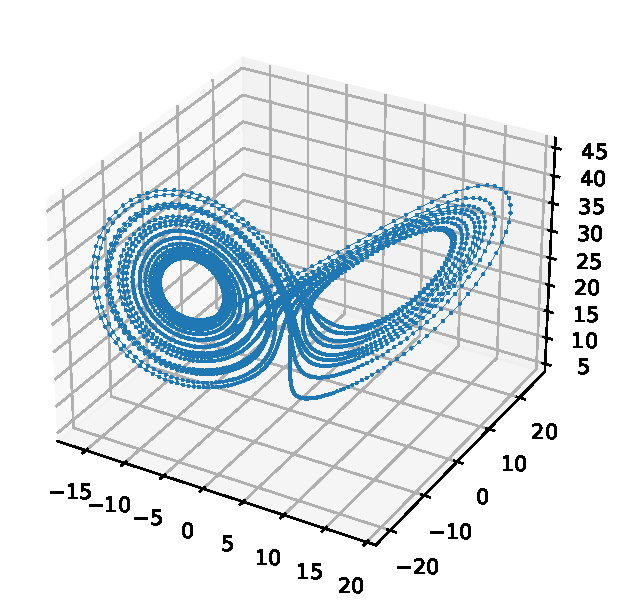
\includegraphics[width=0.27\textwidth]{img/ex1_res}
};
\draw [->] (coef) -- (equation);
\end{tikzpicture}
\end{figure}
\end{frame}


\begin{frame}
\frametitle{Используемые инструменты}

\begin{itemize}
  \item Язык программирования Python
  \item Библиотеки научных вычислений NumPy и SciPy
  \item Библиотека машинного обучения Scikit-learn
  \item Библиотеки построения графиков Matplotlib и Seaborn
\end{itemize}
\end{frame}


\begin{frame}
\frametitle{Архитектура решения}

Разработанное решение реализовано в формате модуля языка Python.
\begin{figure}
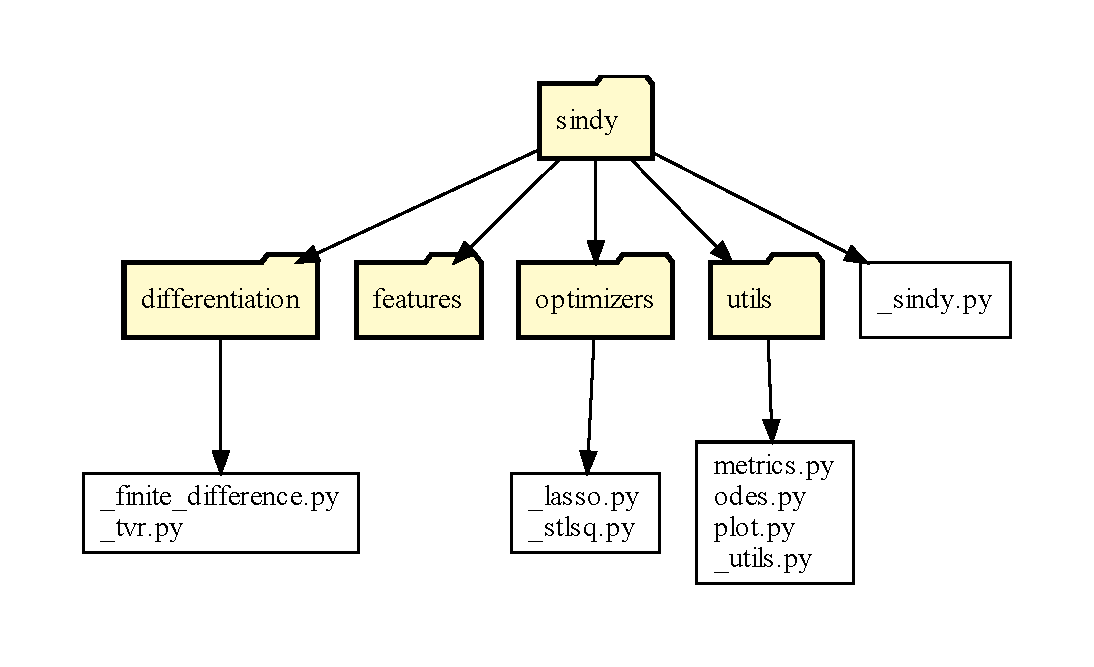
\includegraphics[height=0.8\textheight]{img/tree}
\end{figure}
\end{frame}


\begin{frame}
\frametitle{Работа с данными}

В качестве источника данных использовались различные системы ОДУ:
\begin{figure}
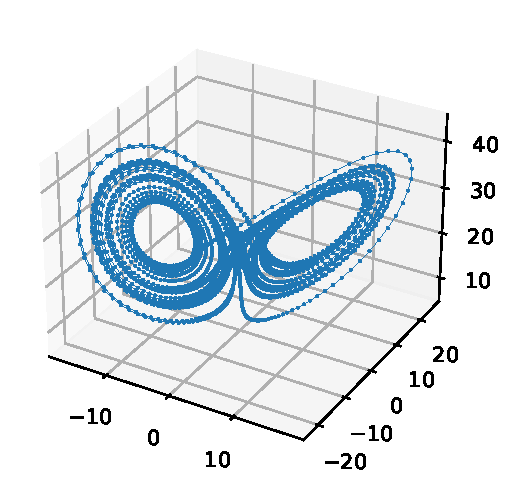
\includegraphics[height=0.38\textheight]{img/lorenz}\hfill
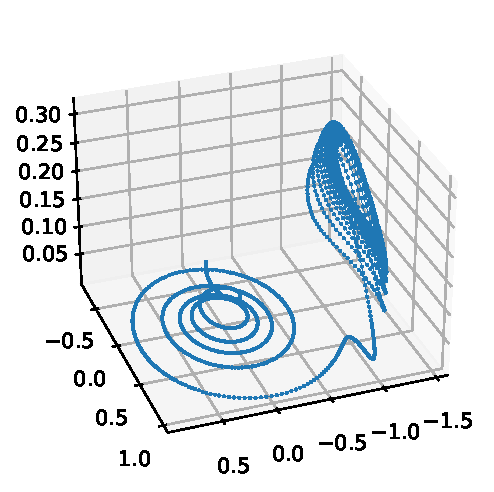
\includegraphics[height=0.38\textheight]{img/fabrab}\hfill
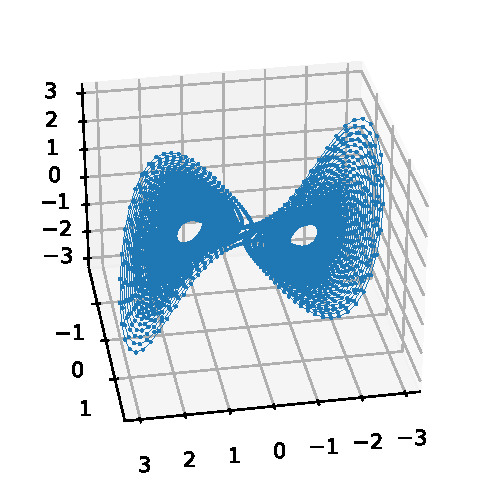
\includegraphics[height=0.38\textheight]{img/moore_spiegel}\hfill
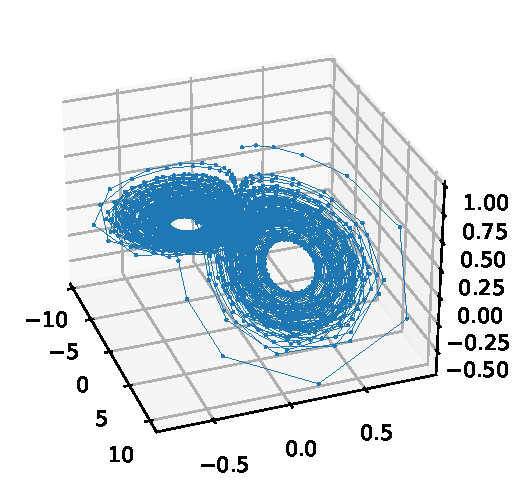
\includegraphics[height=0.38\textheight]{img/vallis}

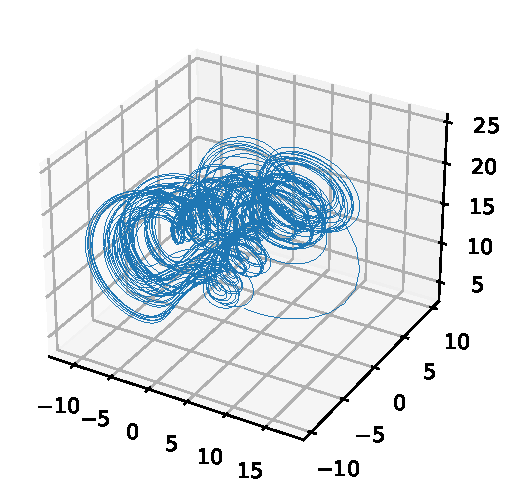
\includegraphics[height=0.38\textheight]{img/generator2}\hfill
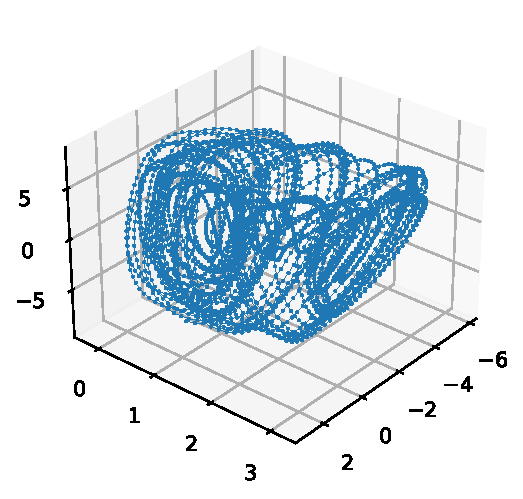
\includegraphics[height=0.38\textheight]{img/torus}\hfill
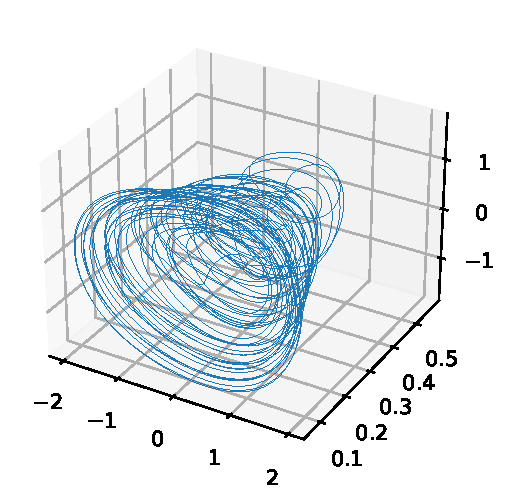
\includegraphics[height=0.38\textheight]{img/aritmic}\hfill
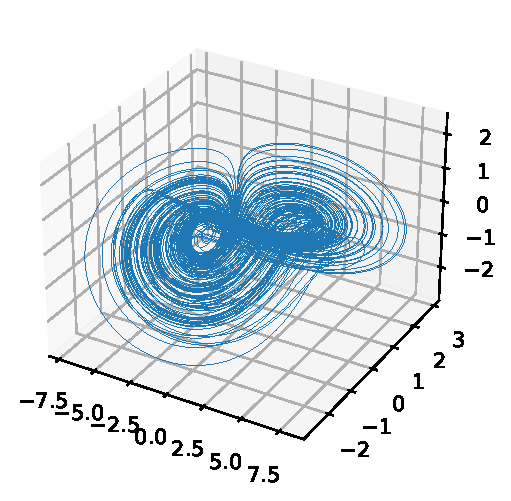
\includegraphics[height=0.38\textheight]{img/simple_3d_model}
\end{figure}
\end{frame}


\begin{frame}
\frametitle{Результаты разработки}
\framesubtitle{Численное дифференцирование зашумленных данных}

\begin{figure}
\includegraphics<1>[width=\textwidth]{img/sin_dif_test}
\includegraphics<2>[height=0.75\textheight]{img/lorenz_dif_test}
\end{figure}
\end{frame}


\begin{frame}
\frametitle{Результаты разработки}
\framesubtitle{Разреженная регрессия}

\begin{figure}
\subfloat[Алгоритм Lasso]{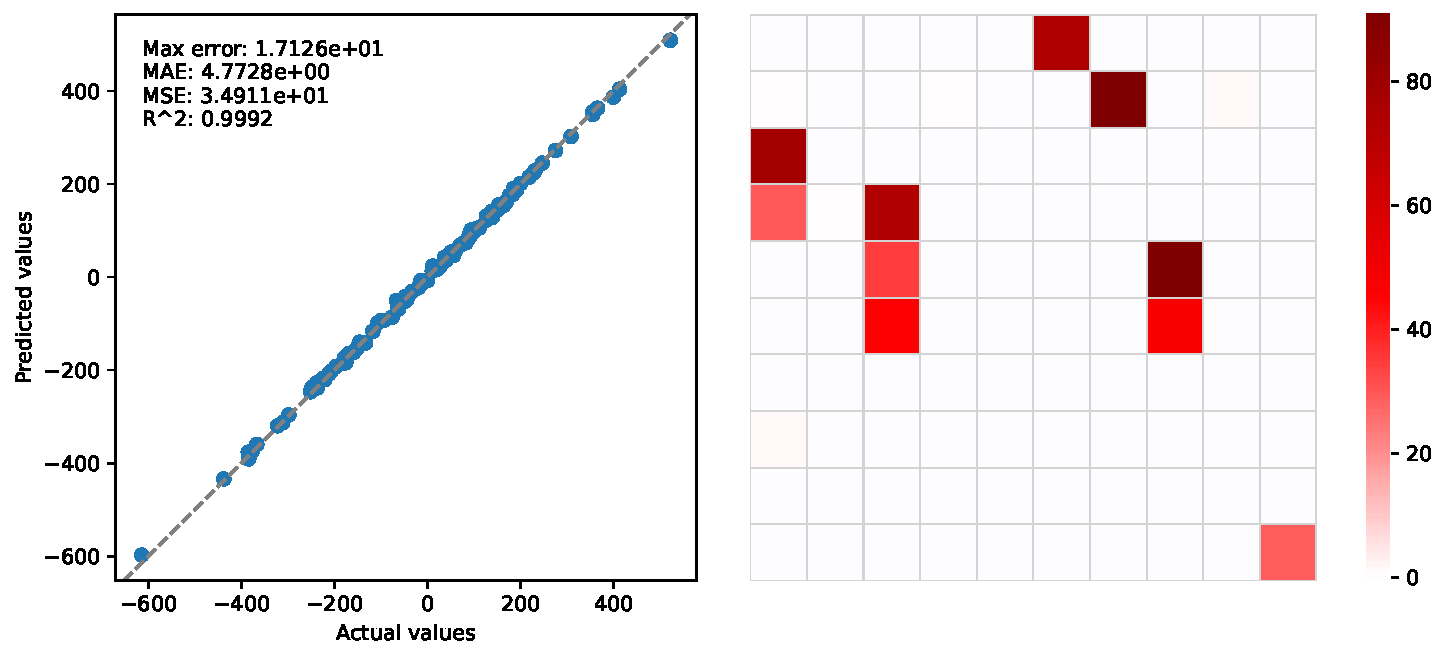
\includegraphics[width=0.49\linewidth]{img/lasso}}\hfill
\subfloat[Алгоритм STLSQ]{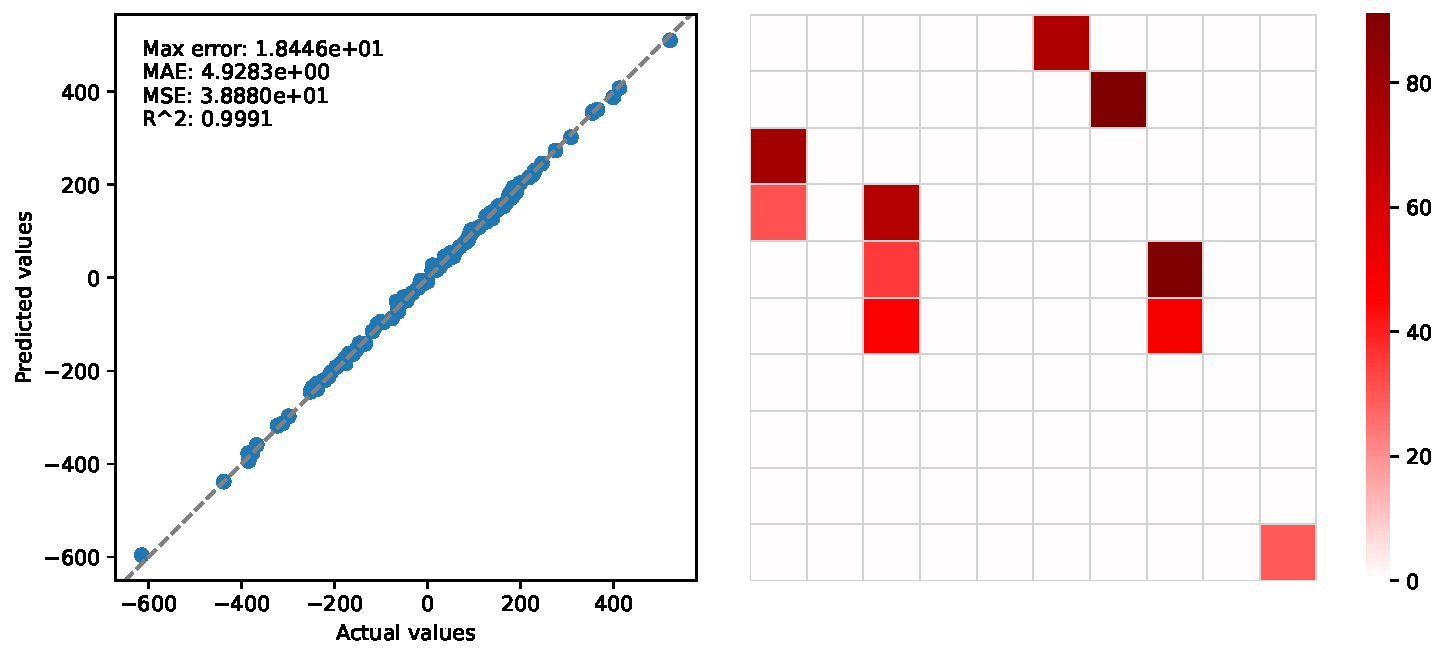
\includegraphics[width=0.49\linewidth]{img/stlsq}}
\end{figure}
\end{frame}


\begin{frame}
\frametitle{Результаты разработки}
\framesubtitle{Структурная идентификация.
\only<1>{Исходная система}\only<2>{Фазовые портреты}\only<3>{Графики метрик}\only<4->{Восстановленные системы}
}

\begin{onlyenv}<1>
\large
\begin{columns}
\column{0.25\textwidth}
  \begin{align*}
  \dot{x} &= \sigma (y - x) \\
  \dot{y} &= x (r - z) - y \\
  \dot{z} &= x y - b z
  \end{align*}
\column{0.25\textwidth}
  \begin{align*}
  \dot{x} &= -10 x + 10 y \\
  \dot{y} &= 28 x - y - x z \\
  \dot{z} &= - 8/3 z + x y
  \end{align*}
\column{0.5\textwidth}
  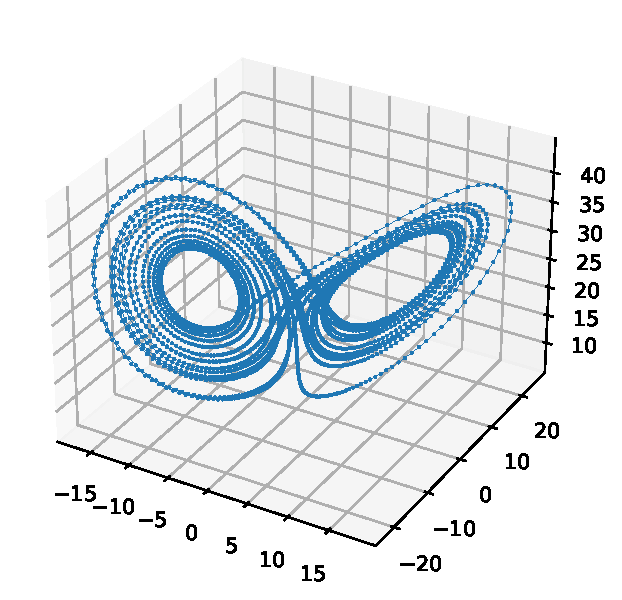
\includegraphics[width=0.93\linewidth]{img/lorenz_big}
\end{columns}
\vfill
\end{onlyenv}

\begin{onlyenv}<2-3>
\begin{figure}
\includegraphics<2>[height=0.8\textheight]{img/lorenz_test}
\includegraphics<3>[height=0.8\textheight]{img/lorenz_scores}
\end{figure}
\end{onlyenv}

\begin{onlyenv}<4>
Уровень шума: $0$
\vfill
\begin{columns}
\column{0.333\textwidth}
  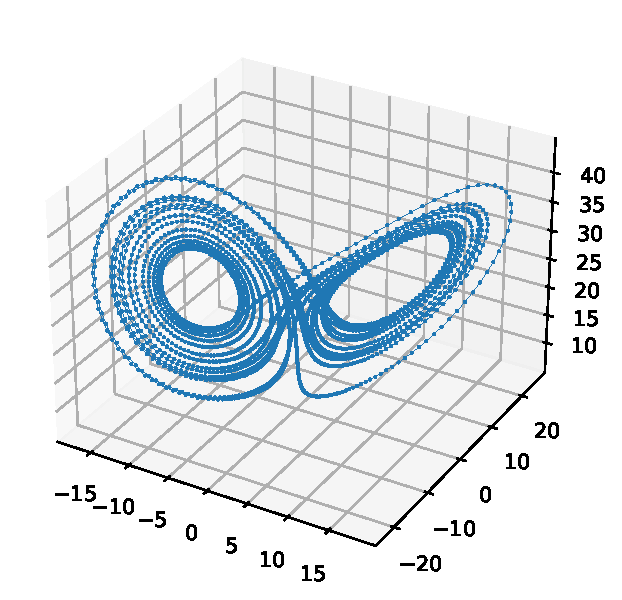
\includegraphics[height=\linewidth]{img/ex1_orig}
\column{0.333\textwidth}
  \begin{align*}
  \dot{x} &= -9.97 x + 9.98 y \\
  \dot{y} &= 27.7 x - 0.89 y - 0.99 x z \\
  \dot{z} &= -2.67 z + 0.99 x y
  \end{align*}
\column{0.333\textwidth}
  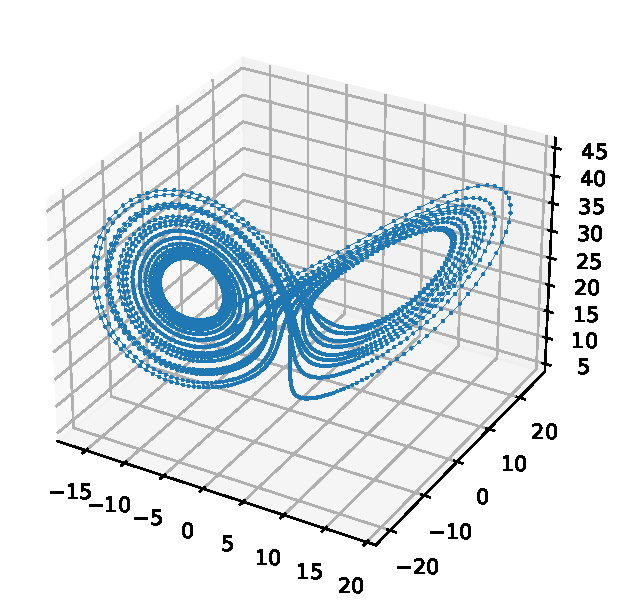
\includegraphics[height=\linewidth]{img/ex1_res}
\end{columns}
\vfill
\begin{center}
  \begin{tabular}{l}
  Потерянных слагаемых: $0$\\
  Лишних слагаемых: $0$\\
  IoU: $1$\\
  \end{tabular}
\end{center}
\end{onlyenv}

\begin{onlyenv}<5>
Уровень шума: $0.01$
\vfill
\begin{columns}
\column{0.333\textwidth}
  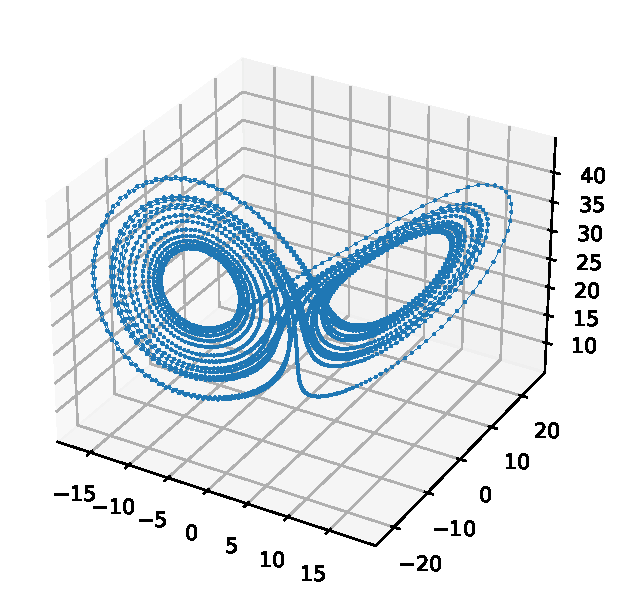
\includegraphics[height=\linewidth]{img/ex2_orig}
\column{0.333\textwidth}
  \begin{align*}
  \dot{x} &= -9.95 x + 9.96 y \\
  \dot{y} &= 27.5 x - 0.87 y - 0.99 x z \\
  \dot{z} &= -2.66 z + 0.99 x y
  \end{align*}
\column{0.333\textwidth}
  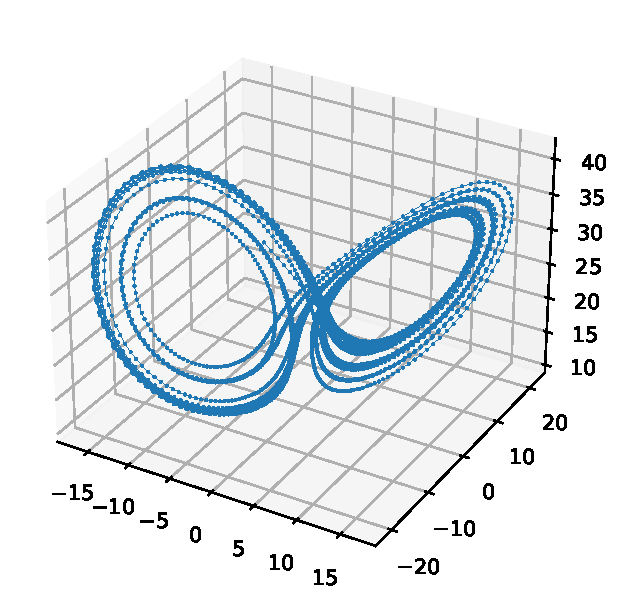
\includegraphics[height=\linewidth]{img/ex2_res}
\end{columns}
\vfill
\begin{center}
  \begin{tabular}{l}
  Потерянных слагаемых: $0$\\
  Лишних слагаемых: $0$\\
  IoU: $1$\\
  \end{tabular}
\end{center}
\end{onlyenv}

\begin{onlyenv}<6>
Уровень шума: $0.1$
\vfill
\begin{columns}
\column{0.333\textwidth}
  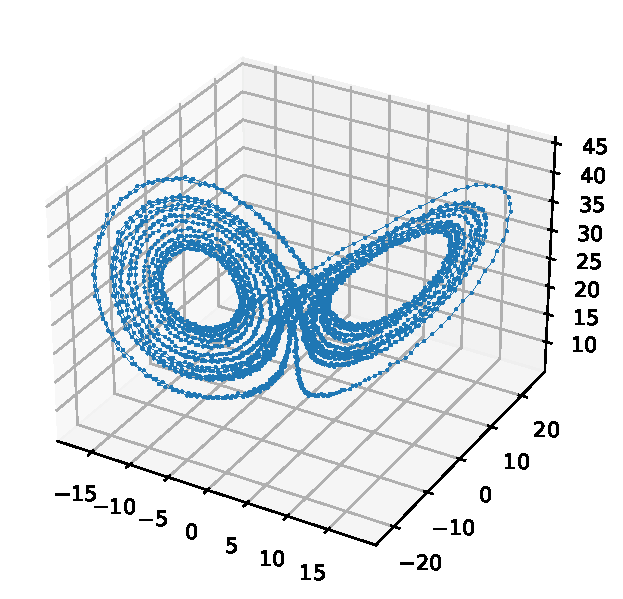
\includegraphics[height=\linewidth]{img/ex3_orig}
\column{0.333\textwidth}
  \begin{align*}
  \dot{x} &= -9.93 x + 9.95 y \\
  \dot{y} &= 27.2 x - 0.8 y - 0.98 x z \\
  \dot{z} &= -2.65 z + 0.99 x y
  \end{align*}
\column{0.333\textwidth}
  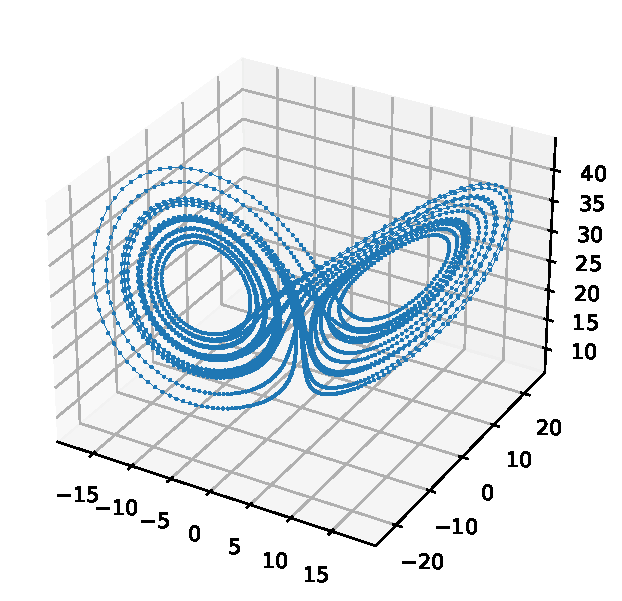
\includegraphics[height=\linewidth]{img/ex3_res}
\end{columns}
\vfill
\begin{center}
  \begin{tabular}{l}
  Потерянных слагаемых: $0$\\
  Лишних слагаемых: $0$\\
  IoU: $1$\\
  \end{tabular}
\end{center}
\end{onlyenv}

\begin{onlyenv}<7>
Уровень шума: $1$
\vfill
\begin{columns}
\column{0.333\textwidth}
  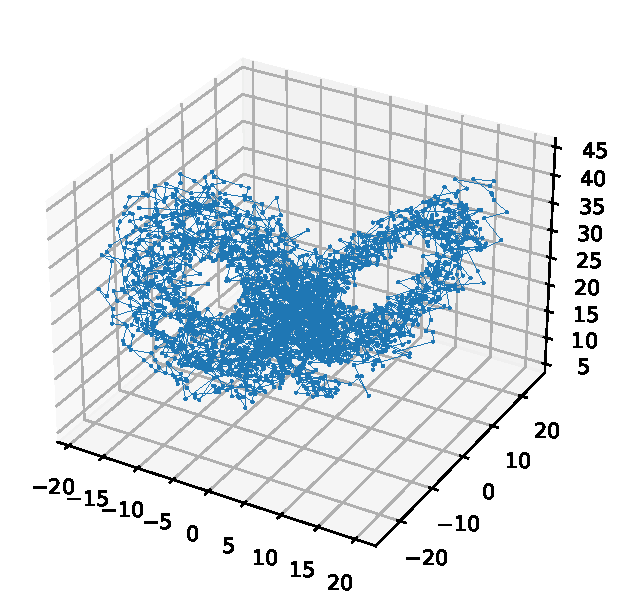
\includegraphics[height=\linewidth]{img/ex4_orig}
\column{0.333\textwidth}
  \begin{align*}
  \dot{x} &= -8.75 x + 8.89 y \\
  \dot{y} &= 21 x + 0.7 y - 0.82 x z \\
  \dot{z} &= -1.65 - 2.43 z + 0.94 x y
  \end{align*}
\column{0.333\textwidth}
  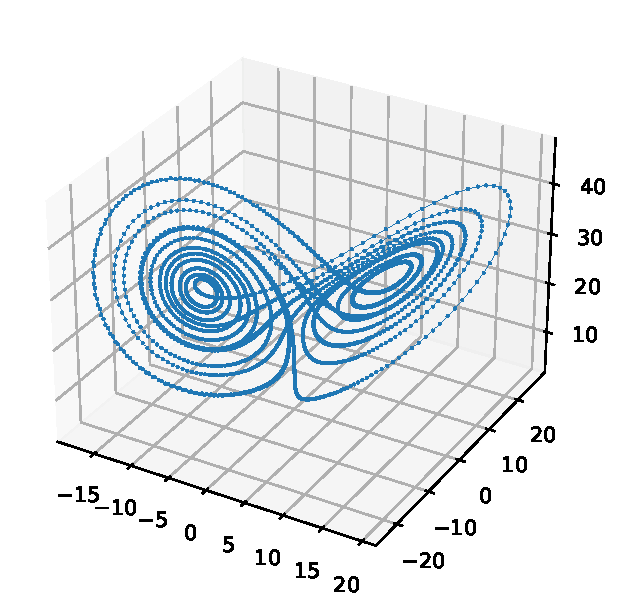
\includegraphics[height=\linewidth]{img/ex4_res}
\end{columns}
\vfill
\begin{center}
  \begin{tabular}{l}
  Потерянных слагаемых: $0$\\
  Лишних слагаемых: $1$\\
  IoU: $0.88$\\
  \end{tabular}
\end{center}
\end{onlyenv}
\end{frame}

\begin{frame}
\frametitle{Оценка результата}

\begin{itemize}
\item Основной результат заключается в том, что идентификация систем ОДУ по шумным данным вполне осуществима.
\begin{itemize}
\item Для этого необходимо иметь подходящий набор функций предполагаемых слагаемых.
\item Для эффективной борьбы с шумом нужна оценка его величины.
\end{itemize}
\item Разработаны рекомендации по использованию как отдельных методов, так и всего алгоритма в целом.
\end{itemize}
\end{frame}


\begin{frame}
\frametitle{Описание программной разработки}

Репозиторий с исходным кодом расположен по адресу \url{https://github.com/iktovr/bachelor-diploma}

\begin{figure}

\includegraphics[height=0.7\textheight]{img/qr-code}
\end{figure}
\end{frame}
\end{document}